
\documentclass[a4paper,10.5pt,oneside]{report}

\usepackage[margin=2.0cm]{geometry}
\usepackage{amsmath,amssymb}
\usepackage{graphicx}
\usepackage{booktabs}
\usepackage{array}
\usepackage{multirow}
\usepackage{caption}
\usepackage{subcaption}
\usepackage{float}
\usepackage{hyperref}
\usepackage[titletoc]{appendix}
\usepackage{tocloft}
\usepackage{listings}

\hypersetup{
    colorlinks=true,
    citecolor=black,
    filecolor=black,
    linkcolor=black,
    urlcolor=black
}

\setcounter{tocdepth}{1}
\setlength{\parindent}{0pt}
\setlength{\parskip}{0.45em}

\begin{document}

\begin{titlepage}
\begin{center}

\vspace*{0.5cm}

% University of Melbourne logo.
% Put the official logo file at figures/uom_banner.pdf

\includegraphics[width=0.3\textwidth]{uom_banner.pdf}\\[0.8cm]

{\Large \textsc{Final Report}}\\[0.7cm]

\rule{\linewidth}{0.5mm}\\[0.45cm]

{\LARGE \bfseries The Art of Scientific Computing:}\\[0.15cm]
{\LARGE \bfseries Respiratory Rates
Determining breathing rates through electrocardiogram data analysis ECG-Derived Respiratory Rate Estimation}\\[0.45cm]

\rule{\linewidth}{0.5mm}\\[0.9cm]

\begin{minipage}[t]{0.46\textwidth}
\begin{flushleft}
\large
\textit{Author:}\\
Guangmei Tang\\[0.25cm]
\textit{Student ID:}\\
\textbf{1562065}
\end{flushleft}
\end{minipage}
\hfill
\begin{minipage}[t]{0.46\textwidth}
\begin{flushright}
\large
\textit{Subject Code:}\\
COMP90072
\end{flushright}
\end{minipage}

\vfill

Faculty of Science\\
The University of Melbourne\\[0.5cm]

{\small \textbf{Submission Date:} []}\\[1.2cm]

{\small \textbf{Subject Coordinator:} A/Prof
Suzie Sheehy}

\end{center}
\end{titlepage}
\clearpage
\pagenumbering{roman}

\chapter*{Summary}
\addcontentsline{toc}{chapter}{Summary}

This report investigates whether respiratory-related information can be
estimated from long-duration electrocardiogram (ECG) recordings. The project
uses the PhysioNet Apnea-ECG database and focuses on developing a clear and
reproducible Python workflow for reading ECG data, interpreting QRS and apnea
annotations, extracting R--R intervals, and analysing their variation over
time.

At the current stage, the ECG waveform and annotation files have been
successfully loaded and aligned on a common time axis. Short ECG segments have
been visualised together with the supplied QRS annotations to confirm that the
annotation locations correspond closely to the R peaks. The next stage of the
project is to construct the R--R interval time series and investigate whether
respiratory-related periodic behaviour can be identified and used to estimate
respiratory rate. Further analysis will compare normal and apnea-labelled
periods and examine the reliability and limitations of the method.

\clearpage

\tableofcontents

\clearpage
\pagenumbering{arabic}
\chapter{Introduction}

\section{Background}

Respiratory rate is the number of complete breathing cycles per minute and is
an important physiological measurement for monitoring respiratory condition
\cite{lung2025}. Changes in breathing rate may provide useful information about
a person's respiratory status, especially during long-term monitoring.

Respiration is normally measured using dedicated respiratory sensors. However,
electrocardiogram (ECG) signals are also commonly recorded over long periods
and contain detailed information about cardiac activity. This raises an
interesting question: whether useful respiratory-related information can be
obtained indirectly from ECG recordings.

This project uses the PhysioNet Apnea-ECG database, which contains
long-duration ECG recordings together with QRS and apnea annotations
\cite{penzel2000}. The availability of both the ECG waveform and its annotations
makes the dataset suitable for developing and testing a reproducible signal
analysis workflow.

From a scientific computing perspective, this problem involves several stages.
The raw ECG data must first be read and interpreted correctly, the annotations
must be aligned with the waveform, useful features must then be extracted, and
the resulting time-series data must be analysed to identify possible
respiratory-related patterns.

\section{ECG and Respiratory Information}

An electrocardiogram records the electrical activity of the heart over time
\cite{ecgsource}. A typical ECG waveform contains several characteristic
components, including the P wave, QRS complex and T wave. In this project, the
QRS complex is especially important because the R peak provides a useful time
marker for each heartbeat.

If two successive R peaks occur at times $t_i$ and $t_{i+1}$, the corresponding
R--R interval is defined as

\begin{equation}
RR_i = t_{i+1} - t_i .
\end{equation}

The R--R interval sequence describes how the time between successive heartbeats
changes over the recording. Since later analysis depends directly on these
intervals, reliable QRS identification is important. Errors in QRS detection
can affect heart-rate variability measurements and other quantities derived
from R--R intervals \cite{weinstein2026}.

The main idea of this project is to investigate whether variation in the
R--R interval sequence contains useful respiratory-related information. The
analysis therefore follows the general pathway

\[
\text{ECG waveform}
\rightarrow
\text{QRS / R peaks}
\rightarrow
\text{R--R intervals}
\rightarrow
\text{time-series analysis}
\rightarrow
\text{respiratory-related information}.
\]

This task is not straightforward because R--R intervals may also vary because
of other physiological changes, abnormal beats, noise, and differences in ECG
morphology. Therefore, changes in R--R intervals cannot simply be interpreted
as respiration, and further time-series analysis is required.

\section{Project Aim}

The main aim of this project is to develop a clear and reproducible Python
workflow for extracting respiratory-related information from ECG recordings.

The first stage of the project focuses on correctly reading and visualising the
ECG waveform together with the supplied QRS and apnea annotations. The QRS
annotations are then used to obtain the timing of successive heartbeats and to
construct an R--R interval time series.

The next stage is to analyse the variation of the R--R intervals and investigate
whether useful respiratory-related patterns can be identified. In particular,
the project aims to determine whether respiratory rate can be estimated from
information derived from the ECG.

After the main ECG-to-respiratory analysis has been established, the extracted
features will also be compared between normal and apnea-labelled periods.
Additional time-series analysis or classification methods may be considered as
extensions if they provide useful information beyond the main analysis.

\chapter{ECG Background and Data Description}

\section{ECG Signal and QRS Complex}

An electrocardiogram (ECG) records the electrical activity of the heart over
time. A typical ECG waveform contains several characteristic components,
including the P wave, QRS complex and T wave \cite{ecgsource}. The P wave is
associated with atrial depolarisation, the QRS complex with ventricular
depolarisation, and the T wave with ventricular repolarisation.

Figure~\ref{fig:ecg_pqrst_rr} illustrates the main components of a typical ECG
waveform and the definition of the R--R interval.

\begin{figure}[H]
    \centering
    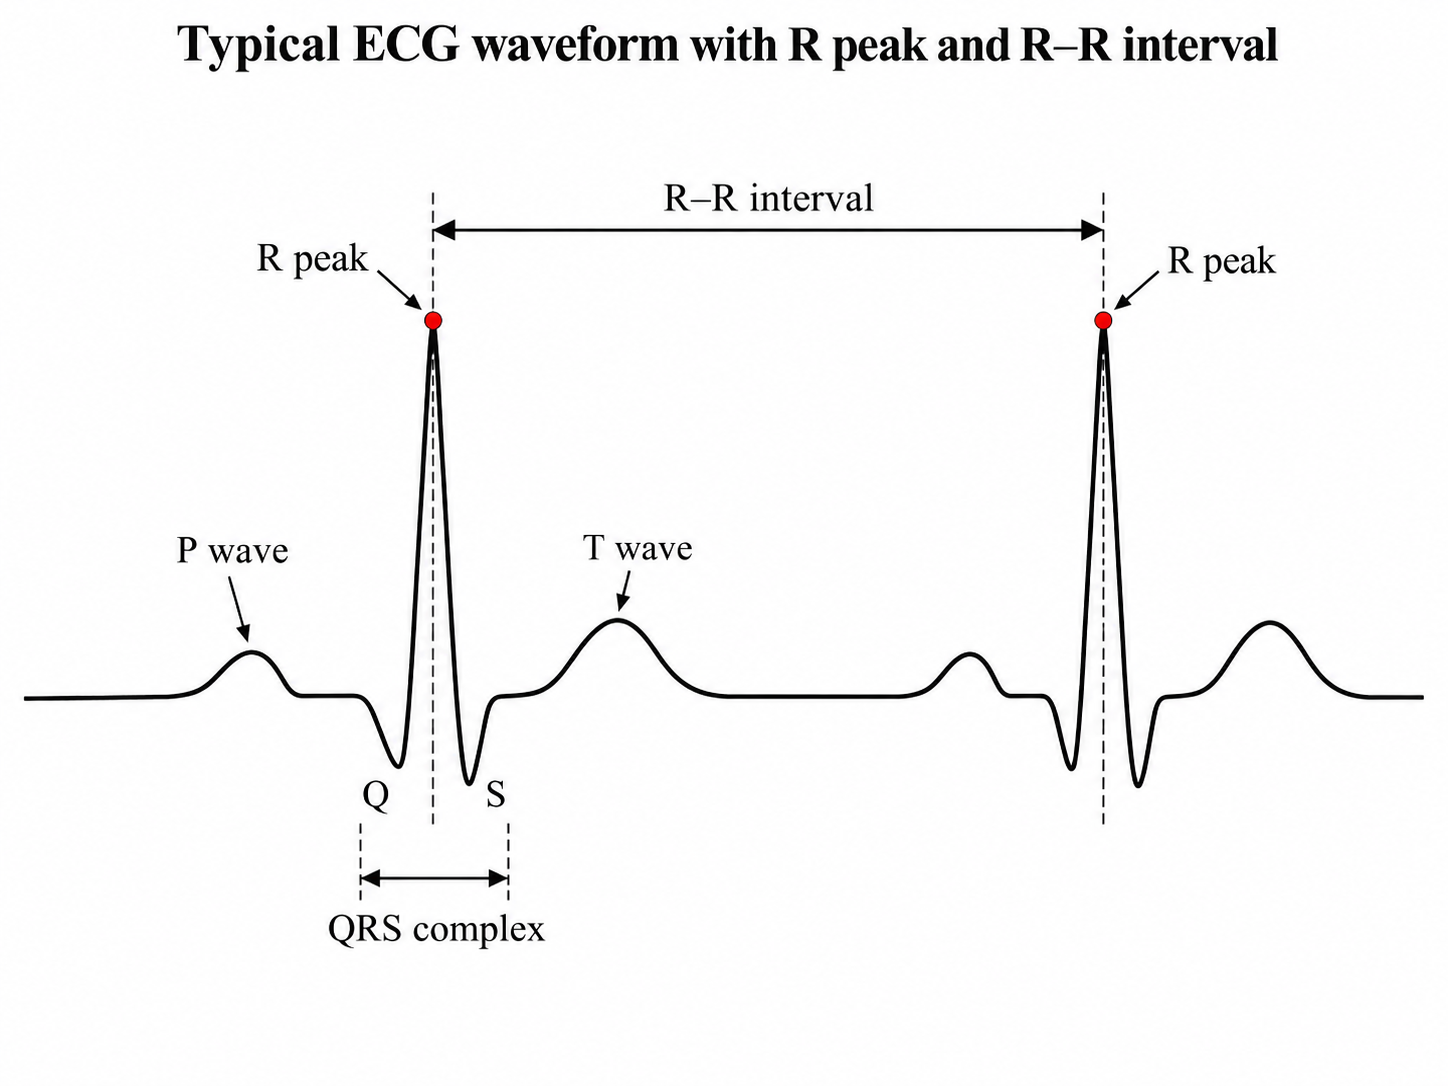
\includegraphics[width=0.6\linewidth]{figuresecg_pqrst_rr.png}
    \caption{Schematic ECG waveform showing the P wave, QRS complex, T wave,
    R peaks and R--R interval. The R peaks are used as heartbeat timing
    references in this project.}
    \label{fig:ecg_pqrst_rr}
\end{figure}

For this project, the QRS complex is the most important part of the ECG waveform
because the R peak provides a clear time marker for each heartbeat. If two
successive R peaks occur at times $t_i$ and $t_{i+1}$, the corresponding
R--R interval is defined as

\begin{equation}
RR_i = t_{i+1} - t_i.
\end{equation}

The R--R interval sequence describes how the timing between successive
heartbeats changes over time. Since the later respiratory analysis depends on
this sequence, reliable identification of QRS complexes is important. Errors in
QRS detection can affect quantities derived from the R--R intervals, including
heart-rate variability measures \cite{weinstein2026}.

Breathing can also influence the timing between heartbeats. Therefore, changes
in the R--R interval sequence may contain useful respiratory-related
information. In this project, the R--R intervals are used as the main
ECG-derived time series for later respiratory analysis.

% Optional conceptual figure
%
% \begin{figure}[H]
%     \centering
%     \includegraphics[width=0.68\linewidth]{figures/ecg_pqrst_rr.pdf}
%     \caption{Schematic ECG waveform showing the P wave, QRS complex,
%     T wave and R--R interval. The R peaks are used as heartbeat timing
%     references in this project.}
%     \label{fig:ecg_pqrst_rr}
% \end{figure}

\section{Apnea-ECG Database}

The data used in this project are obtained from the PhysioNet Apnea-ECG
Database \cite{penzel2000}. The database contains long-duration ECG recordings
together with metadata and annotation files. These annotations make it possible
to study both heartbeat timing and sleep-apnea-labelled periods within the same
recording.

The analysis begins with record \texttt{a01}. Its header file contains the
following information:

\begin{verbatim}
a01 1 100 2957000
a01.dat 16 200 12 0 -12 5827 0 ECG
\end{verbatim}

The first line indicates that record \texttt{a01} contains one signal sampled at
100 Hz, with a total of 2,957,000 samples. Therefore, the total recording length
is approximately

\begin{equation}
\frac{2{,}957{,}000}{100}
=
29{,}570 \text{ s},
\end{equation}

which is approximately 8.21 hours.

Because the recording is several hours long, plotting the complete ECG waveform
at once would make individual beats impossible to inspect clearly. Short time
windows are therefore used for waveform inspection, while longer sections of
the signal are used later for time-series analysis.

\section{WFDB File Structure and Annotations}

The Apnea-ECG data are stored using the WFDB format. Several related files are
used for each record \cite{wfdbguide}:

\begin{itemize}
    \item \texttt{.dat}: contains the ECG waveform data;
    \item \texttt{.hea}: contains the header and metadata required to interpret
    the signal;
    \item \texttt{.qrs}: contains annotations for detected QRS complexes;
    \item \texttt{.apn}: contains annotations for sleep-apnea periods.
\end{itemize}

The waveform and annotation files need to be interpreted on a common time axis.
The QRS annotation locations are stored as sample indices and can be converted
to time in seconds using

\begin{equation}
t = \frac{n}{f_s},
\end{equation}

where $n$ is the sample index and $f_s$ is the sampling frequency.

For record \texttt{a01}, the apnea annotation positions occur every 6000
samples. Since the sampling frequency is 100 Hz,

\begin{equation}
\frac{6000}{100}
=
60 \text{ s}.
\end{equation}

Therefore, one apnea annotation is provided for each minute of the recording.
The annotation symbols used in record \texttt{a01} include \texttt{N} for
normal-labelled periods and \texttt{A} for apnea-labelled periods.

The three main sources of timing information therefore operate on different time
scales. The ECG waveform is sampled at 100 Hz, QRS annotations occur
approximately once per heartbeat, and apnea annotations occur once per minute.
Careful conversion between samples, seconds and minutes is therefore required
before these data can be compared.

\section{Initial ECG and Annotation Inspection}

Before carrying out respiratory analysis, representative ECG segments are first
visualised to check that the waveform and annotation files have been read
correctly.

Figure~\ref{fig:ecg_first10s} shows the first 10 seconds of record
\texttt{a01}. A short time interval is used so that the individual ECG cycles
remain visible. In this segment, repeated large peaks can be clearly observed,
corresponding to the R peaks of successive heartbeats.

\begin{figure}[H]
    \centering
    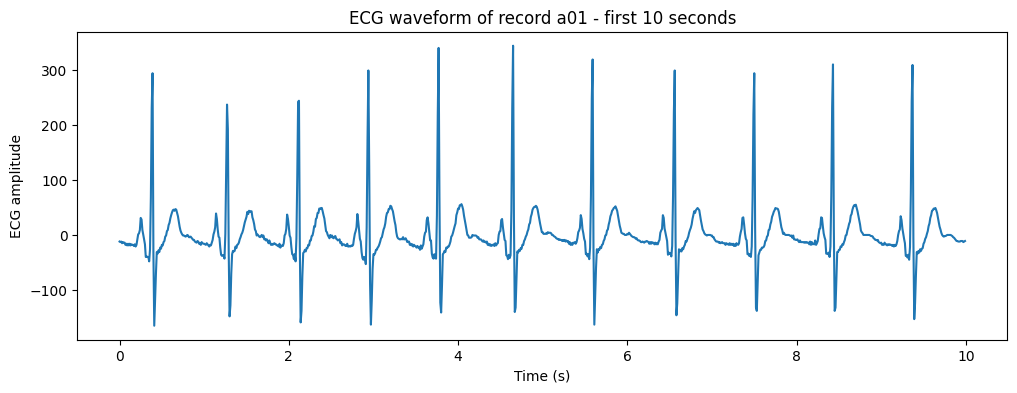
\includegraphics[width=0.82\linewidth]{figuresecg_first10s.png}
    \caption{ECG waveform of record \texttt{a01} over the first 10 seconds.
    The short window allows individual heartbeat cycles and R peaks to be
    inspected clearly.}
    \label{fig:ecg_first10s}
\end{figure}

The supplied QRS annotations are then plotted on the same ECG segment, as shown
in Figure~\ref{fig:ecg_qrs}. The annotation locations align closely with the
large R peaks in the waveform. This provides a basic validation that the ECG
waveform and QRS annotation files have been read consistently.

\begin{figure}[H]
    \centering
    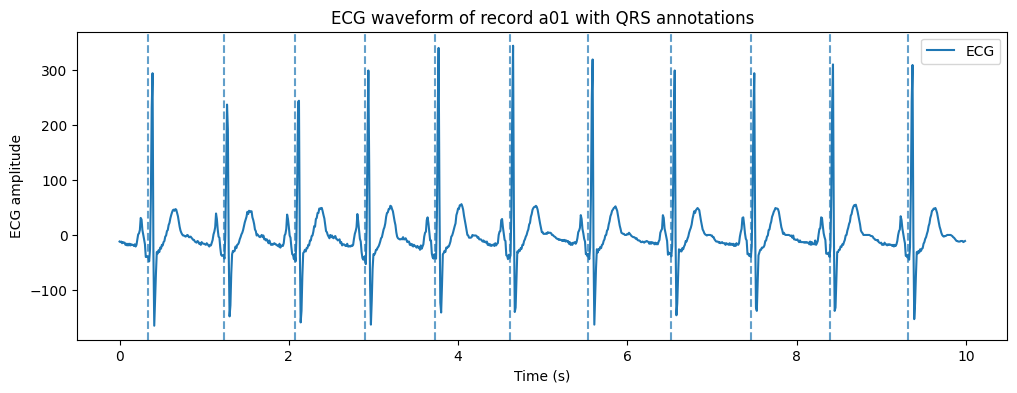
\includegraphics[width=0.82\linewidth]{figuresecg_qrs.png}
    \caption{ECG waveform of record \texttt{a01} with supplied QRS annotations.
    The QRS annotation locations align closely with the R peaks of the ECG
    waveform.}
    \label{fig:ecg_qrs}
\end{figure}

The apnea annotations are also converted onto the ECG time axis. However, since
each apnea label represents a full 60-second interval, plotting several minutes
of ECG together with all QRS annotations produces a very dense figure. Shorter
windows around selected apnea-labelled periods are therefore used later when
the normal and apnea periods are compared.

\chapter{Methodology}

This chapter describes the processing workflow used to move from the raw ECG
recording to ECG-derived time-series information. The current stage of the
analysis focuses on loading and checking the ECG data, reading the supplied QRS
annotations, and constructing the R--R interval sequence. Later stages will use
this sequence to investigate respiratory-related information.

\begin{figure}[H]
    \centering
    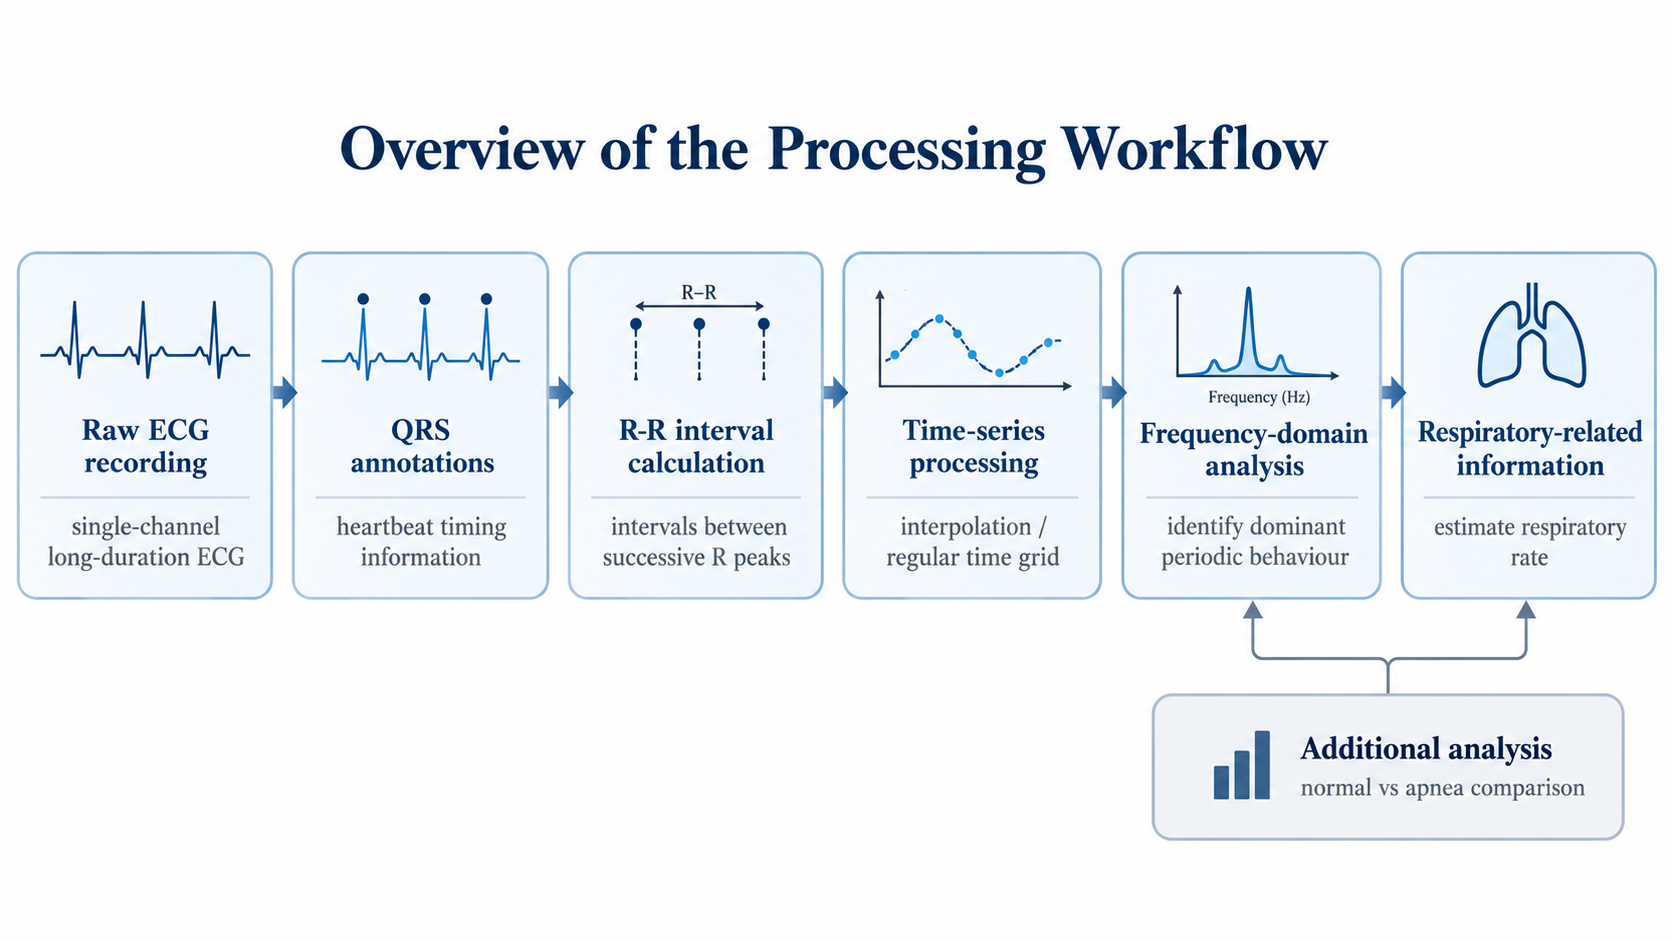
\includegraphics[width=0.8\linewidth]{figuresmethod_workflow.png}
    \caption{Overview of the processing workflow used in this project, from the
    raw ECG recording to R--R interval extraction and respiratory-related
    analysis.}
    \label{fig:method_workflow}
\end{figure}

\section{ECG Reading and Visualisation}

The ECG waveform is read from the Apnea-ECG record using Python. The sampling
frequency is obtained from the corresponding header file. For record
\texttt{a01}, the sampling frequency is

\[
f_s = 100~\text{Hz}.
\]

This means that 100 ECG samples are recorded every second.

A time axis is constructed from the sample indices using

\begin{equation}
t_n = \frac{n}{f_s},
\end{equation}

where $n$ is the sample index and $f_s$ is the sampling frequency.

Because the full recording is more than eight hours long, plotting the entire
signal at once would make individual ECG cycles difficult to distinguish.
Short time windows are therefore used for visual inspection of the waveform.

At the current stage, the raw ECG values are used directly for visualisation.
No conversion to physical units is applied unless the scaling information from
the WFDB header is explicitly used.

\section{QRS and R-Peak Information}

The supplied \texttt{.qrs} annotation file is read using the WFDB tools. Each
annotation gives the sample position of a detected QRS complex.

The annotation sample positions are converted to time in seconds using

\begin{equation}
t_i = \frac{n_i}{f_s},
\end{equation}

where $n_i$ is the sample index of the $i$th QRS annotation.

Before the annotations are used for further analysis, their positions are
visually compared with the ECG waveform. In the inspected segments, the
annotation positions align closely with the large R peaks. This provides a
basic check that the QRS annotations and ECG waveform are being interpreted on
the same time axis.

The supplied QRS annotations are therefore used as the initial reference for
heartbeat timing in the following R--R interval calculation.

\section{R--R Interval Calculation}

For successive R peaks occurring at times $t_i$ and $t_{i+1}$, the R--R
interval is calculated as

\begin{equation}
RR_i = t_{i+1}-t_i.
\end{equation}

The supplied QRS annotations are first converted from sample indices to time in
seconds. The difference between consecutive QRS annotation times is then used
to obtain the R--R interval sequence.

To associate each R--R interval with a time position, the midpoint between the
two corresponding R peaks is used:

\begin{equation}
t_{RR,i} = \frac{t_i+t_{i+1}}{2}.
\end{equation}

This produces a time series of R--R intervals that describes how the time
between successive heartbeats changes throughout the recording.

Because the full record contains a large number of heartbeats, short time
windows are also inspected separately. A five-minute segment is used for
initial inspection because it is long enough to show changes in the R--R
interval sequence while remaining easy to visualise.

\section{R--R Interval Time-Series Processing}

The R--R interval sequence is not sampled at regular time intervals because
successive heartbeats do not occur at exactly equal time spacing. This is an
important issue for later frequency-domain analysis.

Before respiratory-related frequency analysis is applied, the R--R interval
series will therefore be represented on a regular time grid using interpolation.
The interpolated signal can then be analysed using methods that assume evenly
spaced samples.

\section{Respiratory-Related Analysis}

The main aim of the later analysis is to investigate whether periodic variation
in the R--R interval sequence contains respiratory-related information.

A frequency-domain method will be considered to identify dominant periodic
behaviour in the processed R--R signal. If a dominant respiratory-related
frequency $f_r$ is identified in Hz, the corresponding respiratory rate can be
calculated as

\begin{equation}
RR_{\mathrm{resp}} = 60 f_r ,
\end{equation}

where $RR_{\mathrm{resp}}$ is measured in breaths per minute.

The choice of preprocessing method, analysis window and frequency range will be
tested before the final respiratory-rate estimation method is selected.

\section{Additional Analysis}

Additional analyses will only be carried out after the main ECG-to-respiratory
pipeline has been established and tested.

\subsection{Normal and Apnea-Labelled Periods}

The respiratory-related behaviour of the R--R sequence may later be compared
between normal-labelled and apnea-labelled intervals.

\subsection{Apnea Prediction}

Apnea prediction will only be considered if the main respiratory-rate analysis
is working reliably.

\subsection{Alternative Time-Series Methods}

Alternative time-series or time-frequency methods may be tested if they provide
additional information beyond the baseline analysis.

\subsection{Regression or Classification}

Regression or classification methods will be treated as optional extensions
rather than part of the main analysis.
\chapter{Discussion}

\section{Main Findings}

% Directly answer the main research questions.

\section{Reliability of the Analysis}

% Discuss annotation reliability, noise, morphology differences,
% RR outliers and parameter sensitivity.

\section{Interpretation of Respiratory Information}

% Explain what can and cannot be concluded.

\section{Additional Analyses}

% Discuss normal/apnea or ML extensions only if performed.

\section{Limitations}

Important limitations may include:

\begin{itemize}
    \item QRS annotations may contain errors;
    \item ECG morphology varies between records;
    \item R--R interval changes are influenced by factors other than respiration;
    \item parameter choices such as window length may influence the result;
    \item direct respiratory ground truth may not be available for every record.
\end{itemize}

\chapter{Conclusion}

% Keep this concise.
% Summarise the pipeline, main results, robustness,
% additional analyses, limitations and future work.

\begin{appendices}

\chapter{Program Workflow}

% Optional flowchart:
% ECG files -> load waveform/annotations -> visualisation
% -> R peaks -> RR intervals -> respiratory analysis -> additional analysis.

\chapter{Additional Figures and Tables}

% Put useful but non-essential material here.

\end{appendices}

\addcontentsline{toc}{chapter}{References}

\begin{thebibliography}{99}

\bibitem{lung2025}
American Lung Association Editorial Staff,
\textit{Understanding Vital Signs: The Importance of Your Respiratory Rate},
Aug. 19, 2025.
Available at:
\url{https://www.lung.org/blog/respiratory-rate-vital-signs}
(visited Aug. 26, 2026).

\bibitem{penzel2000}
T. Penzel et al.,
``The Apnea-ECG Database,''
\textit{Computers in Cardiology},
vol. 27, pp. 255--258, 2000.
doi: 10.1109/CIC.2000.898505.
Available at:
\url{https://www.physionet.org/content/apnea-ecg/1.0.0/}.

\bibitem{wfdbguide}
PhysioNet,
\textit{WFDB Applications Guide}.
Available at:
\url{https://www.physionet.org/physiotools/wag/}
(visited Aug. 26, 2026).

\bibitem{ecgsource}
Various online contributors,
\textit{Electrocardiography}.
Available at:
\url{https://en.wikipedia.org/wiki/Electrocardiography}
(visited Aug. 26, 2026).

\bibitem{weinstein2026}
A. Weinstein, J. Rodi\~no, and M. Otero,
``Effects of Electrocardiogram QRS Detection Algorithms in Heart Rate Variability Metrics,''
\textit{Scientific Reports},
vol. 16, p. 18589, 2026.
doi: 10.1038/s41598-026-49215-6.
Available at:
\url{https://doi.org/10.1038/s41598-026-49215-6}.

\bibitem{who2022}
World Health Organization,
\textit{Pneumonia in Children},
Nov. 11, 2022.
Available at:
\url{https://www.who.int/news-room/fact-sheets/detail/pneumonia}
(visited Aug. 26, 2026).

\end{thebibliography}

\end{document}
